\documentclass[11pt,a4paper]{article}
\usepackage[utf8]{inputenc}
\usepackage[vietnamese]{babel}
\usepackage{amsmath,amssymb}
\usepackage[version=4]{mhchem}
\usepackage{geometry}
\geometry{top=1.5cm,bottom=1.2cm,left=1.4cm,right=1.4cm,headheight=28pt,headsep=12pt,footskip=18pt}
\usepackage{graphicx}
\usepackage{xcolor}
\usepackage{tabularx}
\usepackage{array}
\usepackage{colortbl}
\usepackage{tikz}
\usepackage{fancyhdr}
\usepackage{enumitem}
\usepackage{multido}
\usepackage{tcolorbox}

\definecolor{hfRed}{HTML}{D32F2F}
\definecolor{hfGreen}{HTML}{8BC390}
\definecolor{mainGreen}{HTML}{2E7D32}
\definecolor{solBlue}{HTML}{1565C0}
\definecolor{tableGreen}{HTML}{E8F5E9}

\usepackage{ex_test}

\pagestyle{fancy}
\fancyhf{}
\renewcommand{\headrulewidth}{0.75pt}
\renewcommand{\headrule}{\hbox to\headwidth{\color{hfGreen}\leaders\hrule height \headrulewidth\hfill}}
\renewcommand{\footrulewidth}{0.75pt}
\renewcommand{\footrule}{\hbox to\headwidth{\color{hfGreen}\leaders\hrule height \footrulewidth\hfill}}

\fancyhead[L]{\small\itshape\color{hfRed}Tài liệu lưu hành nội bộ}
\fancyhead[R]{\small\color{hfRed}Thầy \textbf{TRẦN VĂN THẠNH} - 0777.470.803}

\fancyfoot[L]{\footnotesize\itshape\color{hfRed}CS1: 6/15 Nguyễn Hoàng, P. Kim Long, TP Huế \quad|\quad CS2: 24 Đặng Thái Thân, TP Huế}
\fancyfoot[R]{\small\textbf{\color{hfRed}Trang \thepage}}

\setlength{\parindent}{0pt}
\setlength{\parskip}{2pt}

\begin{document}

\begin{minipage}[t]{0.48\textwidth}
\textbf{SỞ GD\&ĐT TP HUẾ}\\
\textbf{TRƯỜNG THPT NGUYỄN ĐÌNH CHIỂU}\\
\textit{ĐỀ CHÍNH THỨC}\\
\textit{(Đề thi có 03 trang)}
\end{minipage}
\hfill
\begin{minipage}[t]{0.48\textwidth}
\raggedleft
\textbf{\color{hfRed}ĐỀ KIỂM TRA CUỐI HỌC KÌ I}\\
\textbf{NĂM HỌC: 2025 -- 2026}\\
\textbf{Môn: HÓA HỌC -- Khối 12}\\
\textit{Thời gian làm bài: 45 phút (không kể thời gian giao đề)}\\
\textbf{MÃ ĐỀ: 1003}
\end{minipage}

\vspace{4pt}
\noindent
\textit{Họ và tên thí sinh:} \dotfill \textit{Số báo danh:} \dotfill

\vspace{3pt}
\noindent
\textit{\footnotesize Biết: $\ce{H}=1;\ \ce{Cu}=64;\ \ce{Zn}=65;\ \ce{O}=16;\ \ce{C}=12;\ \ce{Na}=23;\ \ce{Ag}=108;\ \ce{N}=14;\ \ce{S}=32;\ \ce{Cl}=35,5;\ \ce{Br}=80$.}

\vspace{3pt}
\hrule color{hfGreen} height 0.5pt

\vspace{4pt}
\noindent
{\color{mainGreen}\textbf{\Large A. PHẦN TRẮC NGHIỆM: (7 điểm)}}

\vspace{3pt}
\noindent
{\color{mainGreen}\textbf{\large PHẦN I: (3,0 điểm) Câu trắc nghiệm nhiều phương án lựa chọn.}}\\
\textit{\small Thí sinh trả lời từ câu 1 đến câu 12, mỗi câu hỏi thí sinh chỉ chọn một phương án.}
\vspace{2pt}

\begin{ex}
Công thức cấu tạo dạng mạch hở của glucose là
\choice
{$\ce{[C6H7O2(OH)3]_n}$}
{$\ce{CH2OH[CHOH]3COCH2OH}$}
{\True $\ce{CH2OH[CHOH]4CHO}$}
{$\ce{CH2OH[CHOH]4CH2OH}$}
\end{ex}
\begin{ex}
Ester X có công thức phân tử $\ce{C4H8O2}$. Thủy phân X trong dung dịch NaOH dư, thu được sản phẩm gồm sodium propionate và alcohol Y. Công thức của Y là
\choice
{\True $\ce{CH3OH}$}
{$\ce{C3H5(OH)3}$}
{$\ce{C3H7OH}$}
{$\ce{C2H5OH}$}
\end{ex}
\begin{ex}
Một học sinh thực hiện ba thí nghiệm ở điều kiện chuẩn và quan sát được các hiện tượng sau:\\
(1) Copper (Cu) kim loại không phản ứng với dung dịch $\ce{Pb(NO3)2}\ 1\text{ M}$.\\
(2) Lead (Pb) kim loại tan trong dung dịch $\ce{AgNO3}\ 1\text{ M}$ và xuất hiện tinh thể Ag.\\
(3) Silver (Ag) kim loại không phản ứng với dung dịch $\ce{Cu(NO3)2}\ 1\text{ M}$.\\
Trật tự nào sau đây thể hiện đúng mức độ khử của ba kim loại?
\choice
{$\text{Cu} > \text{Pb} > \text{Ag}$}
{$\text{Cu} > \text{Ag} > \text{Pb}$}
{\True $\text{Pb} > \text{Cu} > \text{Ag}$}
{$\text{Pb} > \text{Ag} > \text{Cu}$}
\end{ex}
\begin{ex}
Trong điều kiện thích hợp, glucose lên men tạo thành khí $\ce{CO2}$ và chất X. Tên gọi của X là
\choice
{methyl alcohol}
{\True ethyl alcohol}
{lactic acid}
{acetic acid}
\end{ex}
\begin{ex}
Công thức cấu tạo dưới đây là của carbohydrate nào?
\begin{center}
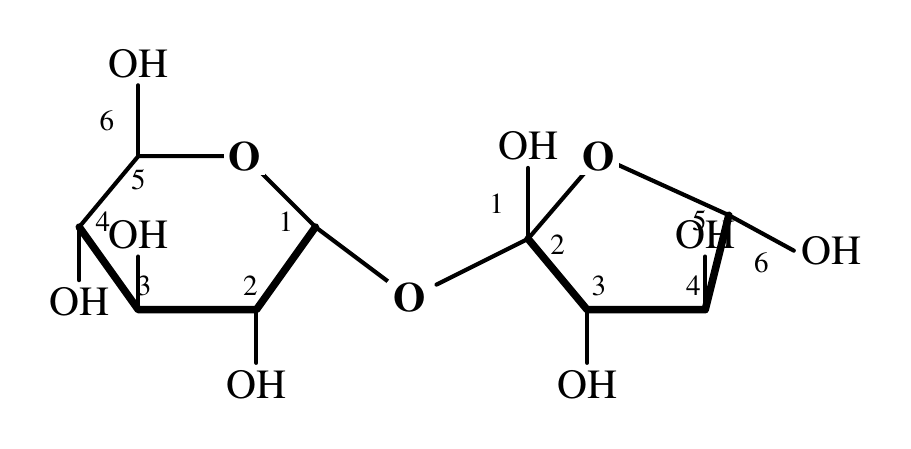
\includegraphics[width=8.0cm]{San_Pham/images_de1003/saccharose_haworth.png}
\end{center}
\choice
{glucose}
{fructose}
{\True saccharose}
{maltose}
\end{ex}
\begin{ex}
Ester có mùi đặc trưng giống mùi táo và có công thức phân tử $\ce{C5H10O2}$. Thủy phân X trong dung dịch NaOH, thu được muối sodium ethanoate và alcohol Y. Oxi hóa không hoàn toàn Y thu được chất Z có phản ứng iodoform. Công thức cấu tạo của X là
\choice
{$\ce{CH3CH2CH2COOCH3}$}
{\True $\ce{CH3COOCH(CH3)2}$}
{$\ce{CH3COOCH2CH2CH3}$}
{$\ce{CH3CH2COOCH2CH3}$}
\end{ex}
\begin{ex}
Dãy chỉ gồm các amino acid có số nhóm amino ($-\ce{NH2}$) bằng số nhóm carboxyl ($-\ce{COOH}$)?
\choice
{\True Gly, Val, Ala}
{Val, Lys, Ala}
{Gly, Ala, Lys}
{Gly, Ala, Glu}
\end{ex}
\begin{ex}
Chất nào sau đây khi đun nóng với dung dịch $\ce{H2SO4}$ loãng thu được sản phẩm có aldehyde?
\choice
{$\ce{CH3-COO-CH2-CH=CH2}$}
{$\ce{CH2=CH-COO-CH2-CH3}$}
{\True $\ce{CH3-COO-CH=CH-CH3}$}
{$\ce{CH3-COO-C(CH3)=CH2}$}
\end{ex}
\begin{ex}
Từ amino acid X và methyl alcohol điều chế được ester Y có công thức phân tử $\ce{C3H7O2N}$. Công thức cấu tạo của amino acid X là
\choice
{\True $\ce{H2NCH2COOH}$}
{$\ce{CH3CH2COOH}$}
{$\ce{H2NCH2COOCH3}$}
{$\ce{CH3CH(NH2)COOH}$}
\end{ex}
\begin{ex}
Chất nào dưới đây không phải là polymer?
\choice
{Tinh bột}
{Cellulose}
{\True Lipid}
{Protein}
\end{ex}
\begin{ex}
Quá trình cộng hợp liên tiếp nhiều phân tử nhỏ giống nhau hoặc tương tự nhau (monomer) tạo thành phân tử lớn (polymer) được gọi là phản ứng
\choice
{trùng ngưng}
{\True trùng hợp}
{tách}
{thế}
\end{ex}
\begin{ex}
Trong các nhận xét dưới đây, nhận xét nào đúng?
\choice
{Tất cả các chất có công thức $\ce{C_n(H2O)_m}$ đều là carbohydrate}
{\True Đa số các carbohydrate có công thức chung $\ce{C_n(H2O)_m}$}
{Phân tử các carbohydrate đều có ít nhất 6 nguyên tử carbon}
{Tất cả các carbohydrate đều có công thức chung $\ce{C_n(H2O)_m}$}
\end{ex}
\vspace{4pt}
\noindent
{\color{mainGreen}\textbf{\large PHẦN II: (2,0 điểm) Câu trắc nghiệm đúng sai.}}\\
\textit{\small Thí sinh trả lời từ câu 1 đến câu 2. Trong mỗi ý a), b), c), d) ở mỗi câu, thí sinh chọn đúng hoặc sai.}
\vspace{2pt}

\begin{ex}
Cho sơ đồ phản ứng sau:
\begin{align*}
\ce{X}\ (\ce{C4H8O2}) + \ce{H2O} &\xrightarrow{\ce{H+}, t^\circ} \ce{Y} + \ce{Z} \\
\ce{Y} + \ce{C3H5(OH)3} &\xrightarrow{\ce{H2SO4}\ \text{đặc}, t^\circ} \ce{T} \\
\ce{Z} &\xrightarrow{\text{men giấm}} \ce{Y} \\
\ce{Z} + \ce{HCOOH} &\xrightarrow{\ce{H2SO4}\ \text{đặc}, t^\circ} \ce{W}
\end{align*}
Biết rằng X, Y, Z, T, W là các hợp chất hữu cơ khác nhau; T chỉ chứa một loại nhóm chức.
\choiceTF
{Y có trong nọc độc của kiến}
{Phần trăm khối lượng của nguyên tố oxygen trong T là $36,36\%$}
{\True Công thức cấu tạo của W là $\ce{HCOOC2H5}$}
{\True Z có trong thành phần của nước rửa tay khô có tác dụng diệt khuẩn}
\end{ex}
\begin{ex}
Cho các chất có công thức cấu tạo sau:
$\ce{H2NCH2COOH}$ (1); $\ce{C2H5COOH}$ (2); $\ce{C2H5NH2}$ (3); $\ce{H2NCH2CH2CH(NH2)COOH}$ (4); $\ce{C6H5NH2}$ (5).
\choiceTF
{\True Có 4 chất tác dụng được với dung dịch HCl}
{Có 1 chất tác dụng được với ethanol khi có mặt xúc tác $\ce{H2SO4}$ đặc, đun nóng}
{\True Có 3 chất tác dụng được với dung dịch NaOH}
{\True Có 2 chất vừa tác dụng được với acid vừa tác dụng được với base}
\end{ex}
\vspace{4pt}
\noindent
{\color{mainGreen}\textbf{\large PHẦN III: (2,0 điểm) Câu trắc nghiệm yêu cầu trả lời ngắn.}}\\
\textit{\small Thí sinh trả lời từ câu 1 đến câu 4. Thí sinh điền kết quả vào ô trả lời tương ứng.}
\vspace{2pt}

\begin{ex}
Cao su lưu hóa có $2\%$ sulfur (S) về khối lượng. Có bao nhiêu mắt xích isoprene có một cầu disulfide ($\ce{-S-S-}$)? Giả thiết rằng S đã thay thế cho H ở cầu methylene ($-\ce{CH2}-$) trong mạch cao su.
\hfill \textbf{Trả lời:} \dotfill
\end{ex}
\begin{ex}
Thủy phân hoàn toàn $1\text{ mol}$ peptide mạch hở X, thu được $2\text{ mol}$ Gly, $2\text{ mol}$ Ala và $1\text{ mol}$ Val. Mặt khác, thủy phân không hoàn toàn X, thu được hỗn hợp các amino acid và các peptide (trong đó có Gly-Ala-Val). Số công thức cấu tạo phù hợp với tính chất của X là bao nhiêu?
\hfill \textbf{Trả lời:} \dotfill
\end{ex}
\begin{ex}
Cho các polymer sau: polybuta-1,3-diene, poly(vinyl acetate), polystyrene, nylon-6,6 và poly(phenol formaldehyde). Số polymer được điều chế bằng phản ứng trùng ngưng là bao nhiêu?
\hfill \textbf{Trả lời:} \dotfill
\end{ex}
\begin{ex}
Thuỷ phân $4,4\text{ gam}$ ethyl acetate bằng $300\text{ mL}$ dung dịch NaOH $0,2\text{M}$. Sau khi phản ứng xảy ra hoàn toàn, cô cạn dung dịch, thu được $m\text{ gam}$ chất rắn khan. Giá trị của $m$ là bao nhiêu?
\hfill \textbf{Trả lời:} \dotfill
\end{ex}
\vspace{4pt}
\noindent
{\color{mainGreen}\textbf{\Large B. PHẦN TỰ LUẬN: (3 điểm)}}

\vspace{3pt}

\noindent
\textbf{Câu 1. (1,0 điểm)} Hợp chất X có công thức phân tử trùng với công thức đơn giản nhất, vừa tác dụng được với acid vừa tác dụng được với base trong điều kiện thích hợp. Trong phân tử X, thành phần phần trăm khối lượng của các nguyên tố C, H, N lần lượt bằng $40,449\%$; $7,865\%$ và $15,73\%$; còn lại là oxygen. Khi cho $4,45\text{ gam}$ X phản ứng hoàn toàn với một lượng vừa đủ dung dịch NaOH (đun nóng) thu được $4,85\text{ gam}$ muối khan. Xác định công thức cấu tạo của X.

\vspace{2pt}
\multido{\i=1+1}{8}{\noindent\dotfill\\}

\vspace{4pt}
\noindent
\textbf{Câu 2. (1,0 điểm)} Nhúng một thanh Zn vào $100\text{ mL}$ dung dịch $\ce{CuSO4}$, sau một thời gian phản ứng lấy thanh Zn ra khỏi dung dịch, làm khô và đem cân thấy khối lượng thanh Zn giảm $0,01\text{ gam}$. Cho dung dịch loãng NaOH dư vào dung dịch sau phản ứng thu được $0,49\text{ gam}$ kết tủa. Tính nồng độ mol của dung dịch $\ce{CuSO4}$ ban đầu.

\vspace{2pt}
\multido{\i=1+1}{8}{\noindent\dotfill\\}

\vspace{4pt}
\noindent
\textbf{Câu 3. (1,0 điểm)} Để sản xuất $10\text{ L}$ cồn y tế $70^\circ$ người ta cần lên men tối thiểu $m\text{ gam}$ glucose. Biết hiệu suất của quá trình lên men là $80\%$, khối lượng riêng của ethanol là $0,789\text{ g/mL}$. Giá trị của $m$ là bao nhiêu?

\vspace{2pt}
\multido{\i=1+1}{7}{\noindent\dotfill\\}

\vspace{8pt}
\begin{center}
\textbf{---------- HẾT ----------}
\end{center}

\end{document}
